\section{Problem 4: Implementation of METRICSTICS}

\subsection{Tech Stack}
To implement METRICSTICS, Python was used as the programming language, specifically Python 3. It is dynamically typed and garbage-collected. It is also able to support multiple programming paradigms, such as structured (procedural), object-oriented and functional programming. \cite{python} For the development of this application, the object-oriented programming paradigm was used.

For the GUI, a library called Tkinter was used, which is a Python binding to the Tk GUI toolkit, Python's de facto standard GUI. \cite{tkinter}

To calculate descriptive statistics, users of METRICSTICS are able to either:
\begin{enumerate}
    \item Generate random values
    \item Upload a CSV file
\end{enumerate}

\begin{figure}[!htb]
    \begin{center}
    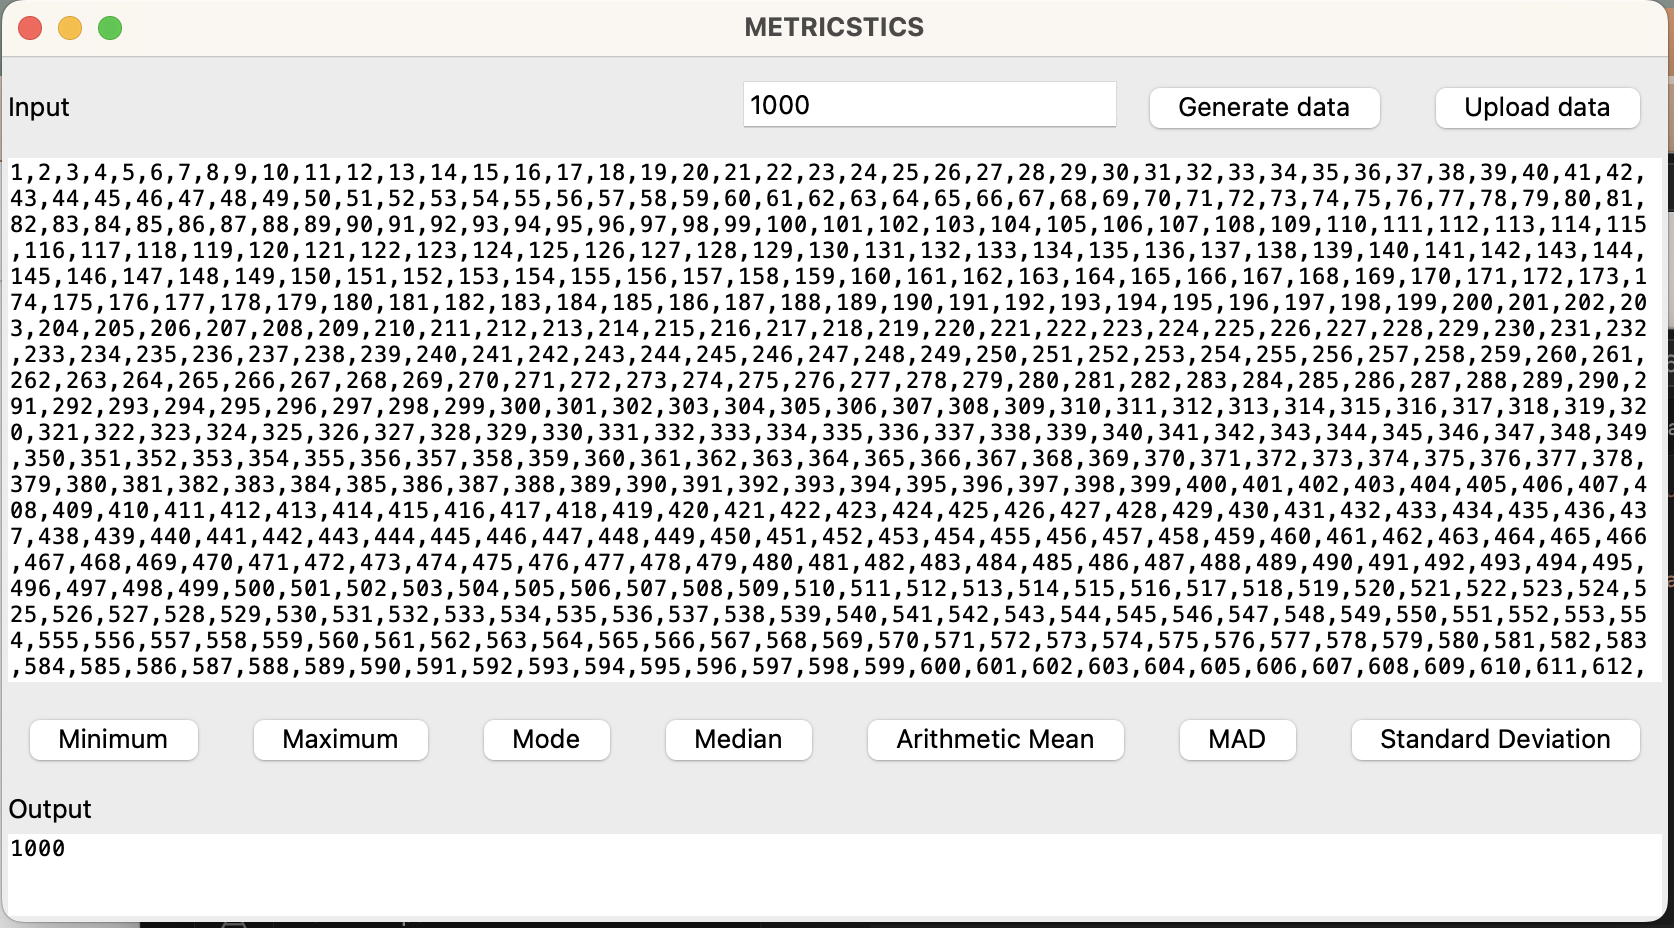
\includegraphics[width=12cm]{images/gui.png} % 
    \end{center}
    \caption{METRICSTICS Application}
\end{figure}

\begin{figure}[ht]
    \begin{center}
    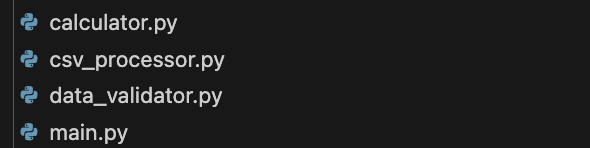
\includegraphics[width=8cm]{images/pythonclasses.png} % 
    \end{center}
    \caption{Python Classes}
\end{figure}

\begin{figure}
    \begin{center}
    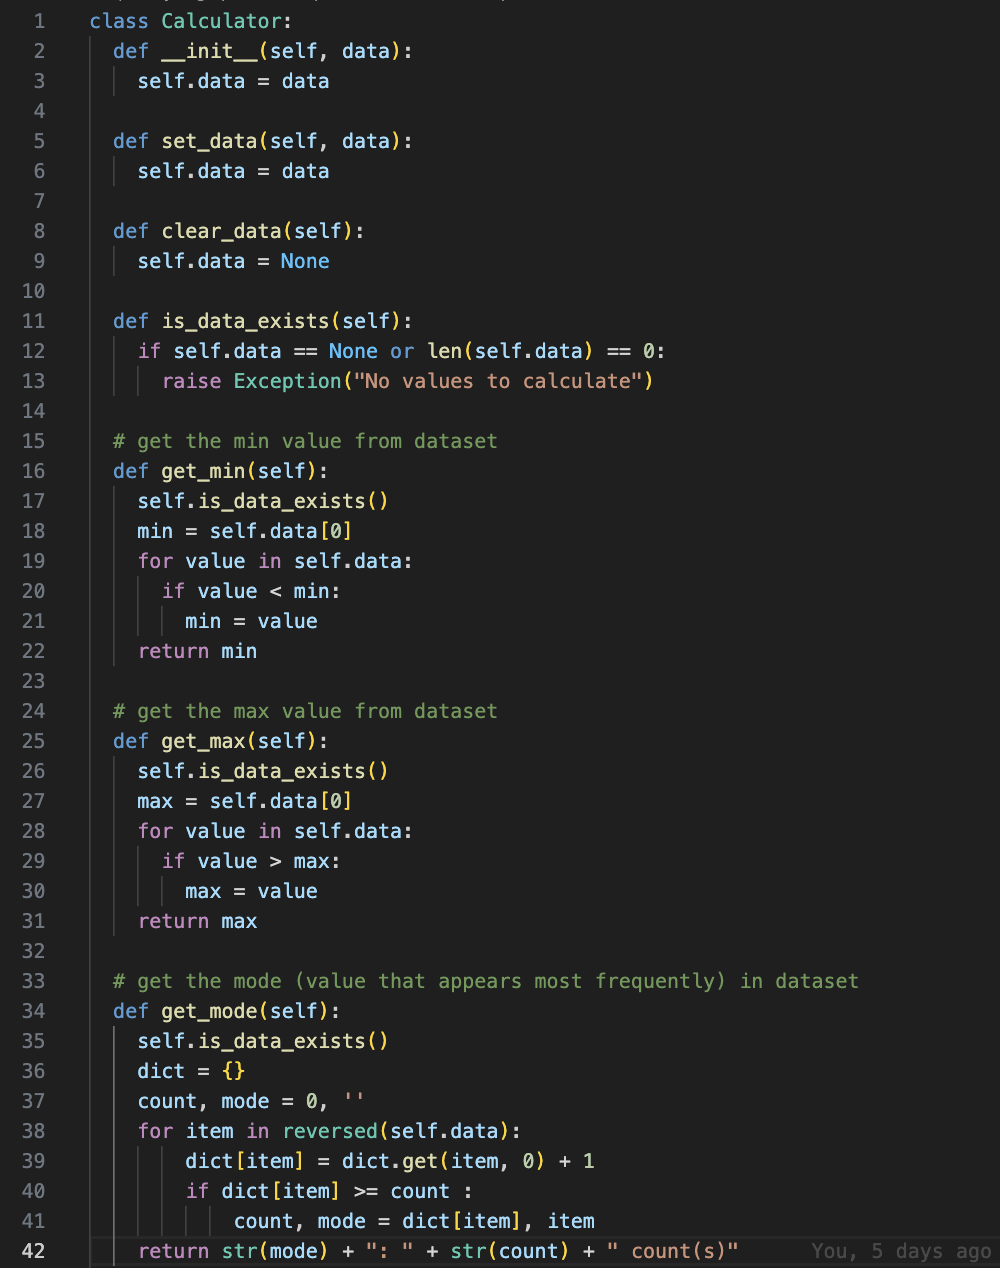
\includegraphics[width=12cm]{images/codesample.png}
    \end{center}
    \caption{Sample Code - Object-oriented Paradigm}
\end{figure}

\pagebreak

\subsection{Tests}
Input files that have been used for the tests can be found in the 'input' folder in the repository, while the output files of the corresponding inputs can be found in the 'output' folder. The examples below provide a summary of tests performed. Detailed and more extensive tests can be found in the repository folder.

\begin{enumerate}
    \item[--]Input files with the prefix 'input\{x\}\_\{xxx\}.csv' were used to test the csv upload function (labelled as the 'Upload data' button)
    \item[--]Input files with the prefix 'random\{x\}.csv' were values generated from the button labelled as 'Generate data'. These values were copied into a csv file for tracing and verification purposes for the input and their corresponding outputs produced.
    \item[--]Output files are prefixed with the input file name and the functions they have performed so that they can be easily identified and verified.
    \item[--]For example, the 'Mininum' screenshot for 'random1.csv' is named as 'random1\_min.png', the `Standard Deviation` for 'input1\_sequential.csv' is named as 'input1\_standarddeviation.png', etc
\end{enumerate}


\begin{longtable}{|l|l|}
\hline
\textbf{Test: Input 1} & Input from input1\_sequential.csv \\
\hline
Min &   \raisebox{-\totalheight}{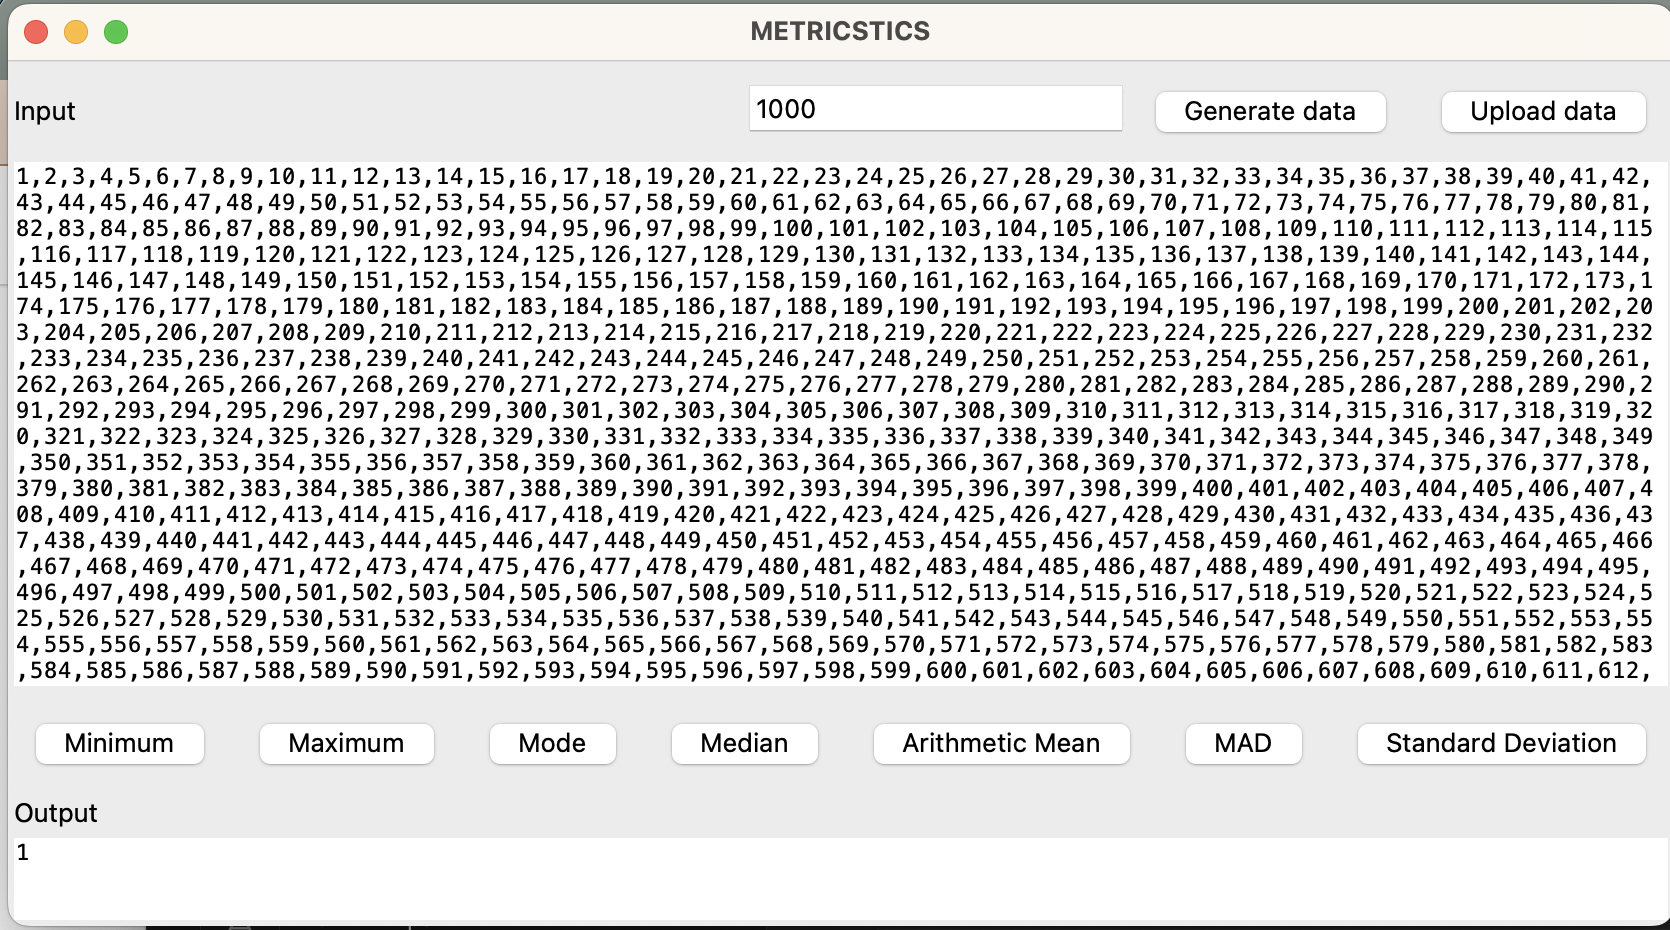
\includegraphics[width=11cm\textwidth]{images/input1_min.png}}\\
\hline
Max &   \raisebox{-\totalheight}{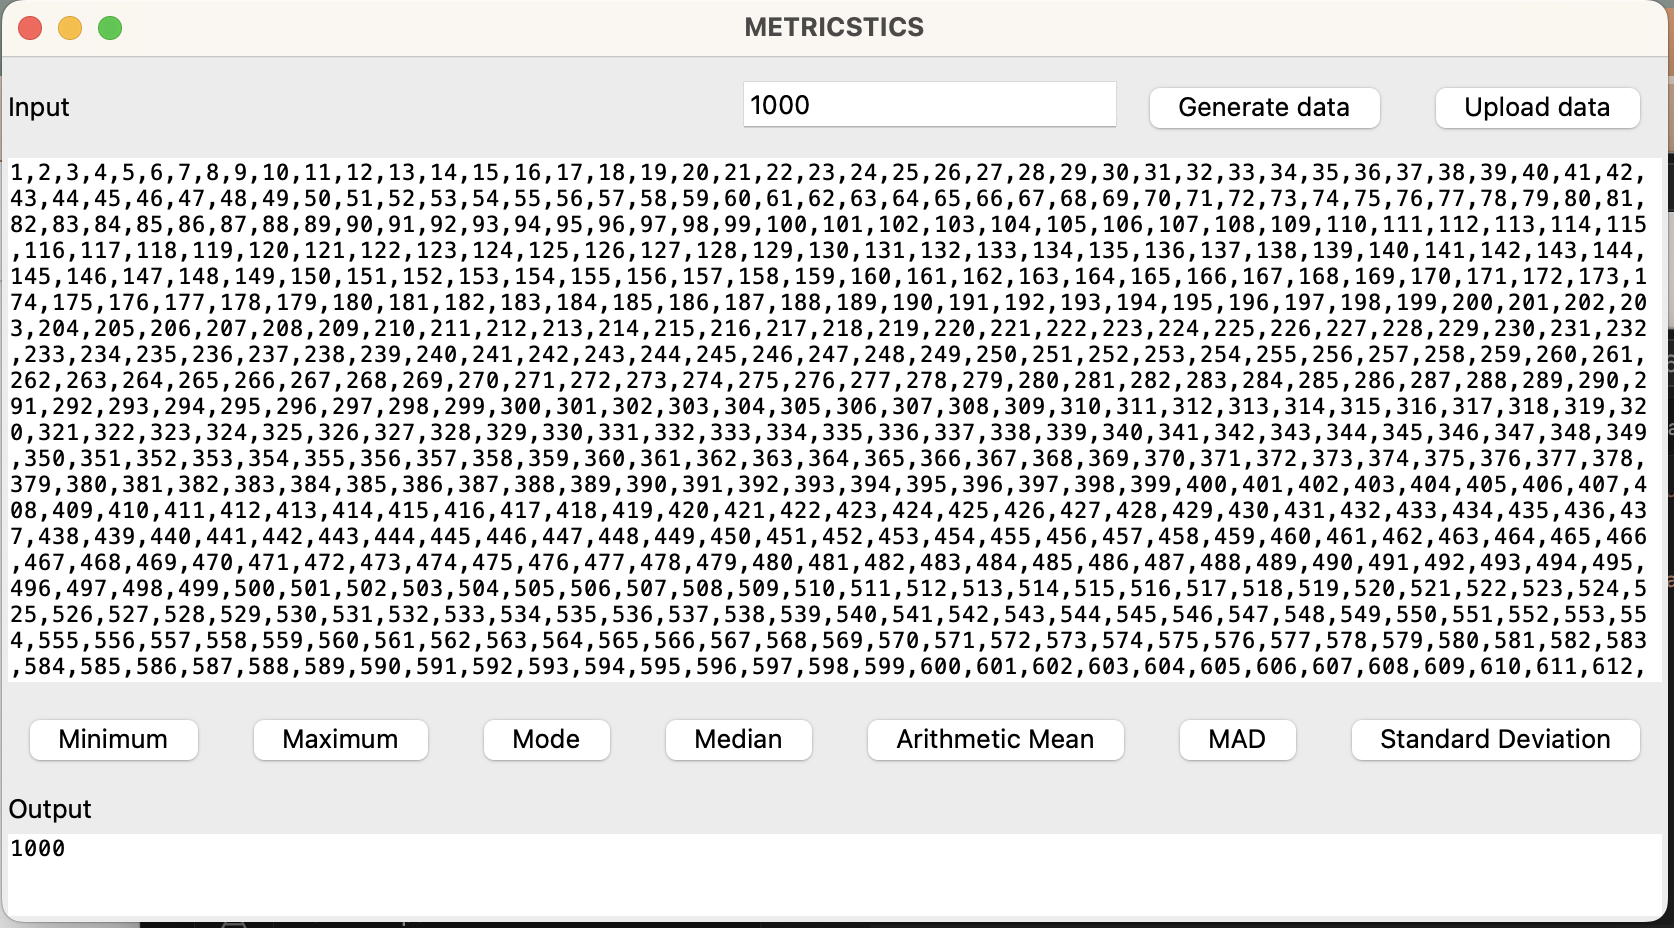
\includegraphics[width=11cm\textwidth]{images/input1_max.png}}\\
\hline
Mode &   \raisebox{-\totalheight}{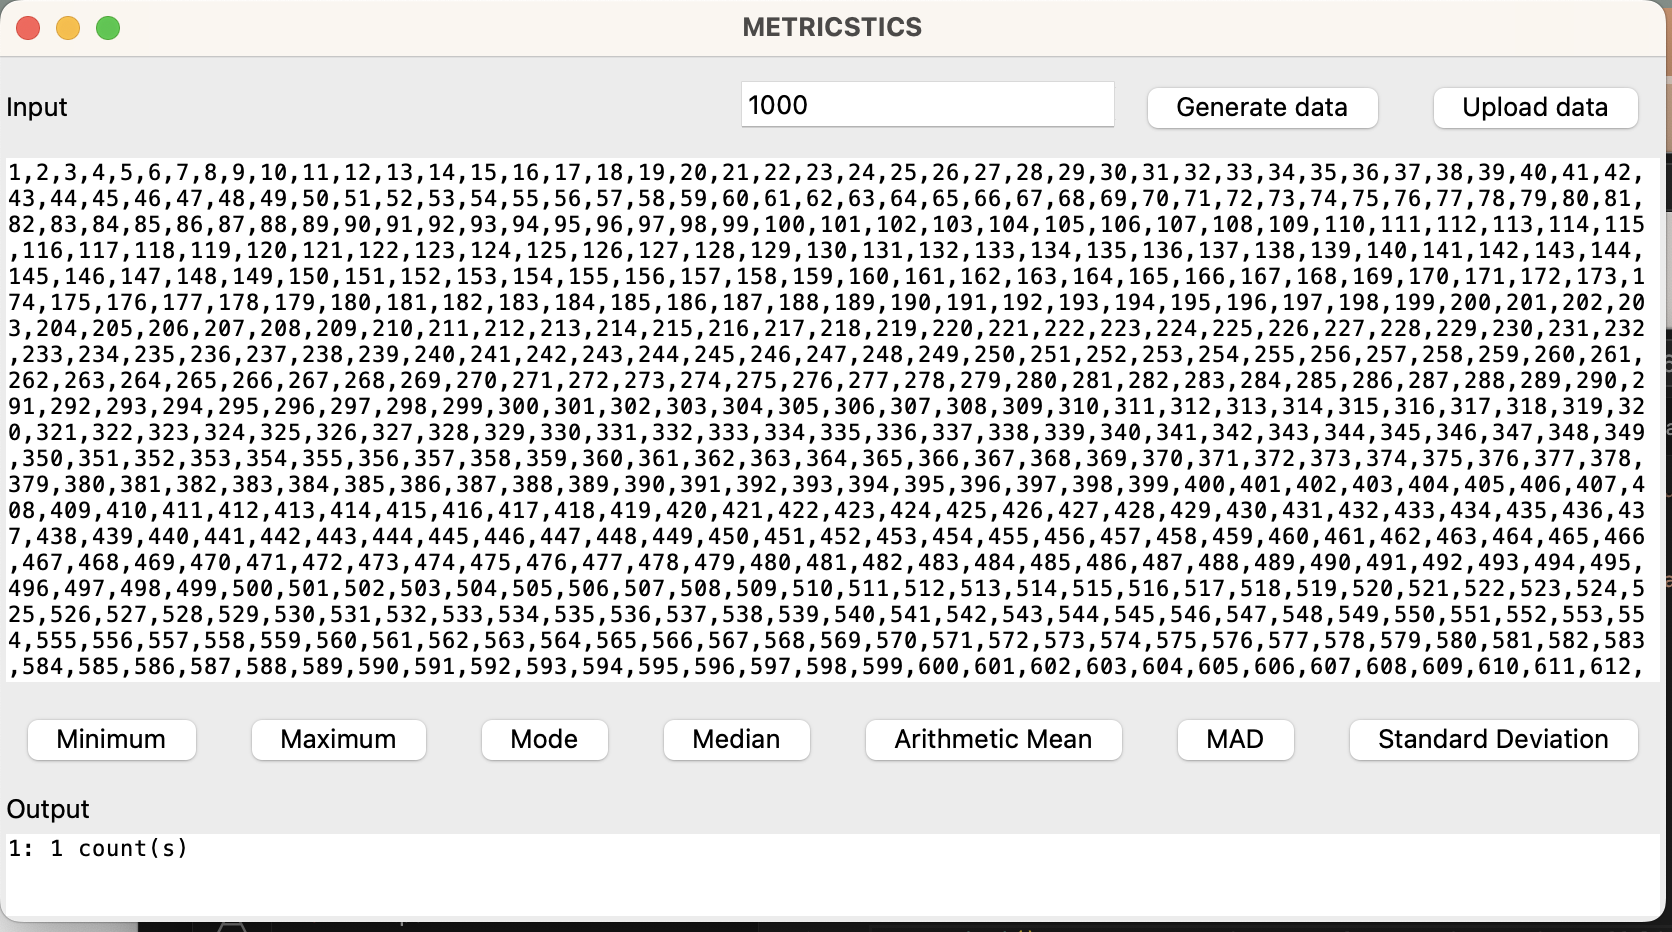
\includegraphics[width=11cm\textwidth]{images/input1_mode.png}}\\
\hline
Median &   \raisebox{-\totalheight}{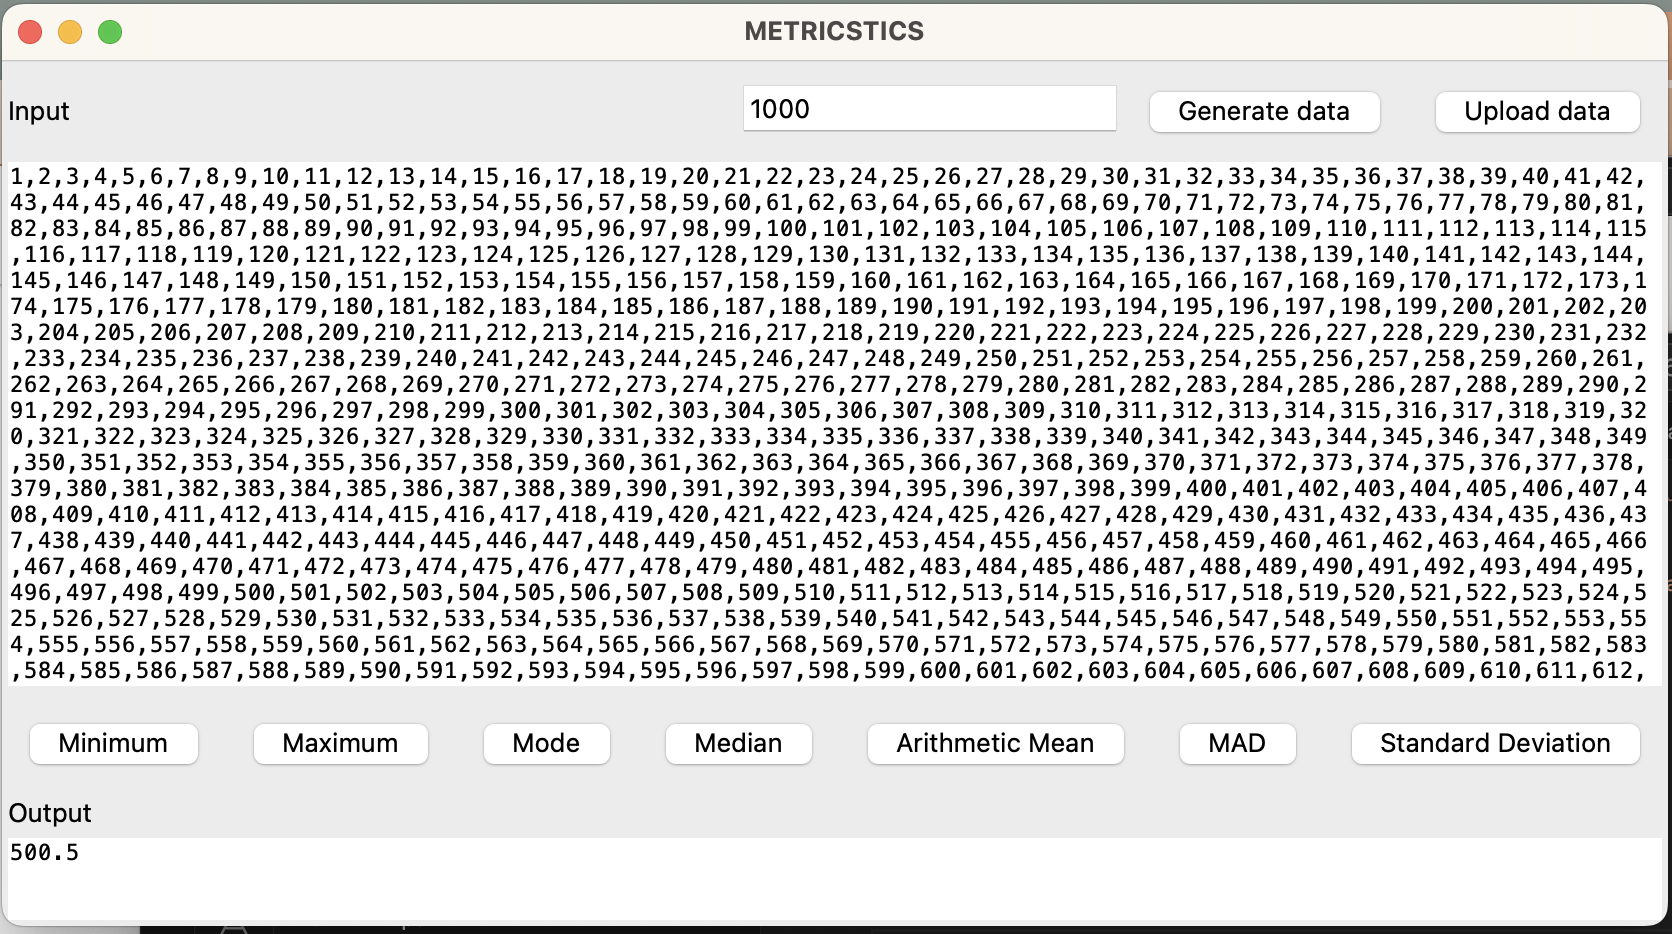
\includegraphics[width=11cm\textwidth]{images/input1_median.png}}\\
\hline
MAD &   \raisebox{-\totalheight}{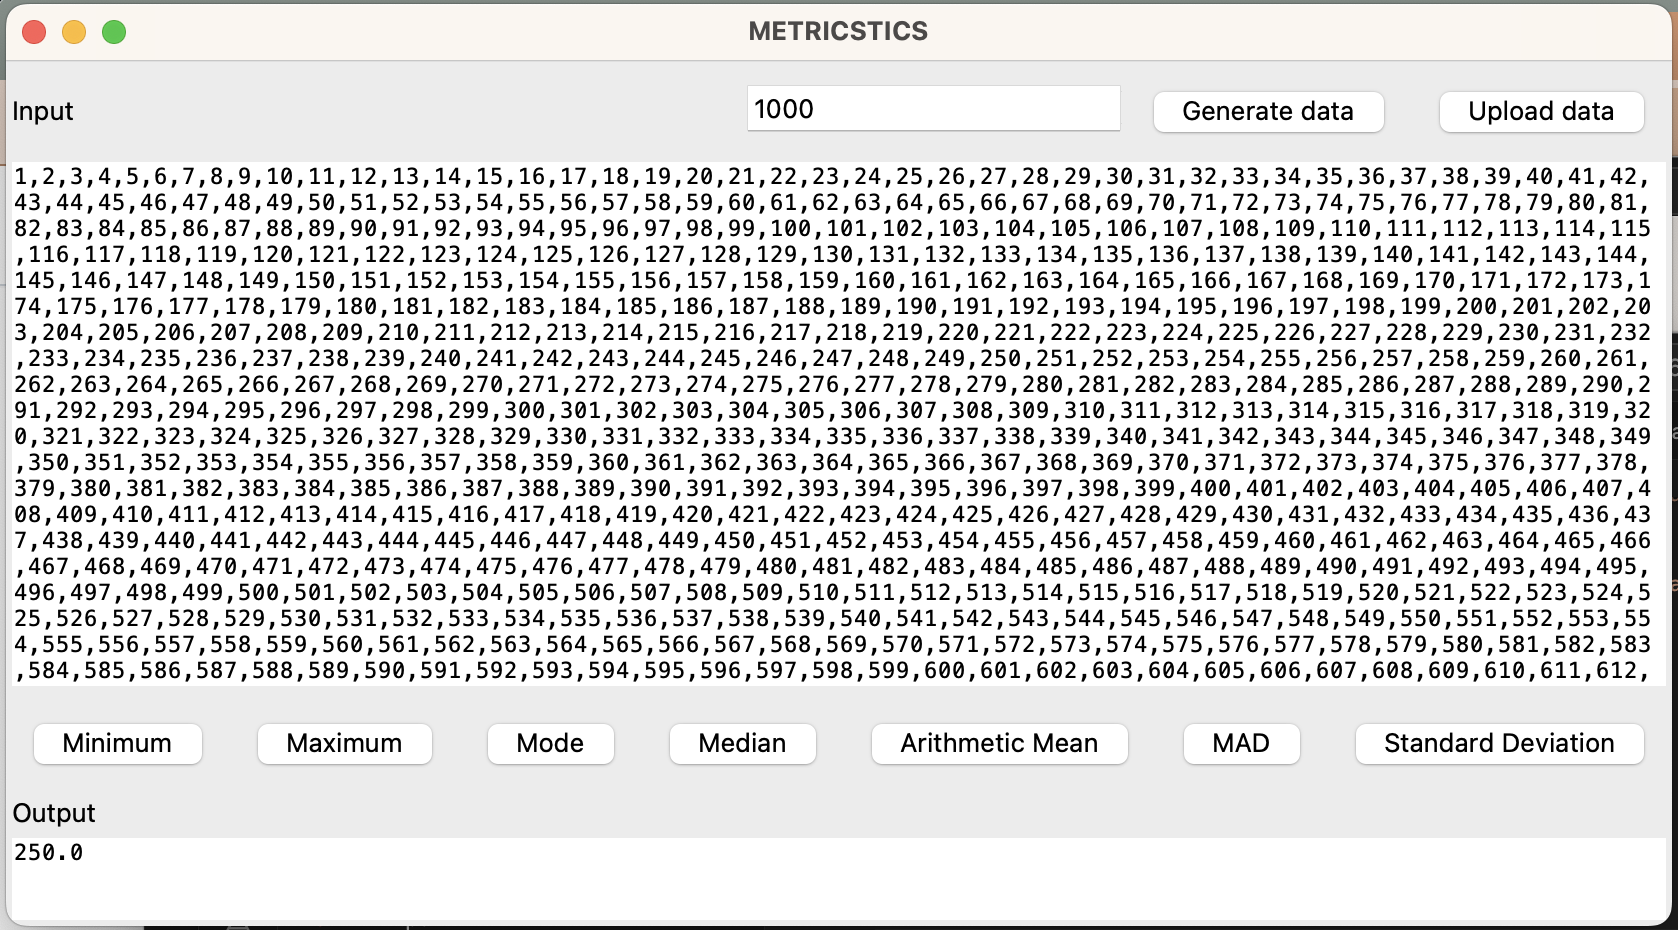
\includegraphics[width=11cm\textwidth]{images/input1_mad.png}}\\
\hline
Standard Deviation &   \raisebox{-\totalheight}{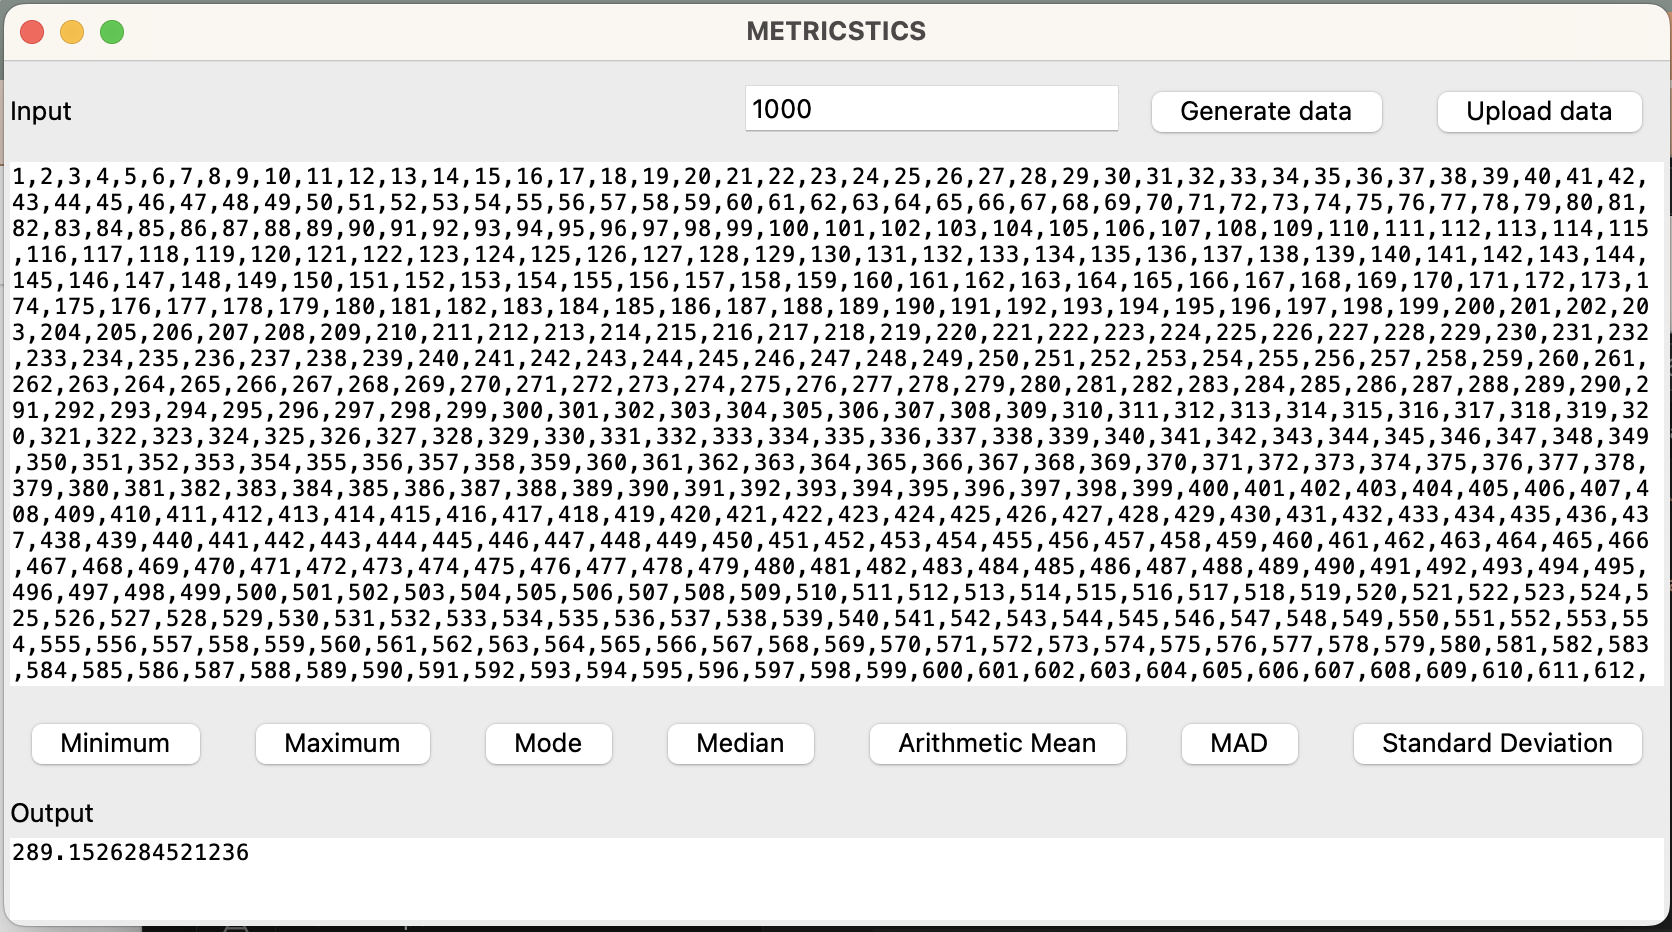
\includegraphics[width=11cm\textwidth]{images/input1_standarddeviation.png}}\\
\hline
\end{longtable}

\begin{longtable}{|l|l|}
\hline
\textbf{Test: Random 1} & Input from clicking on 'Generate Data' (Generated values are saved into 'random1.csv') \\
\hline
Min &   \raisebox{-\totalheight}{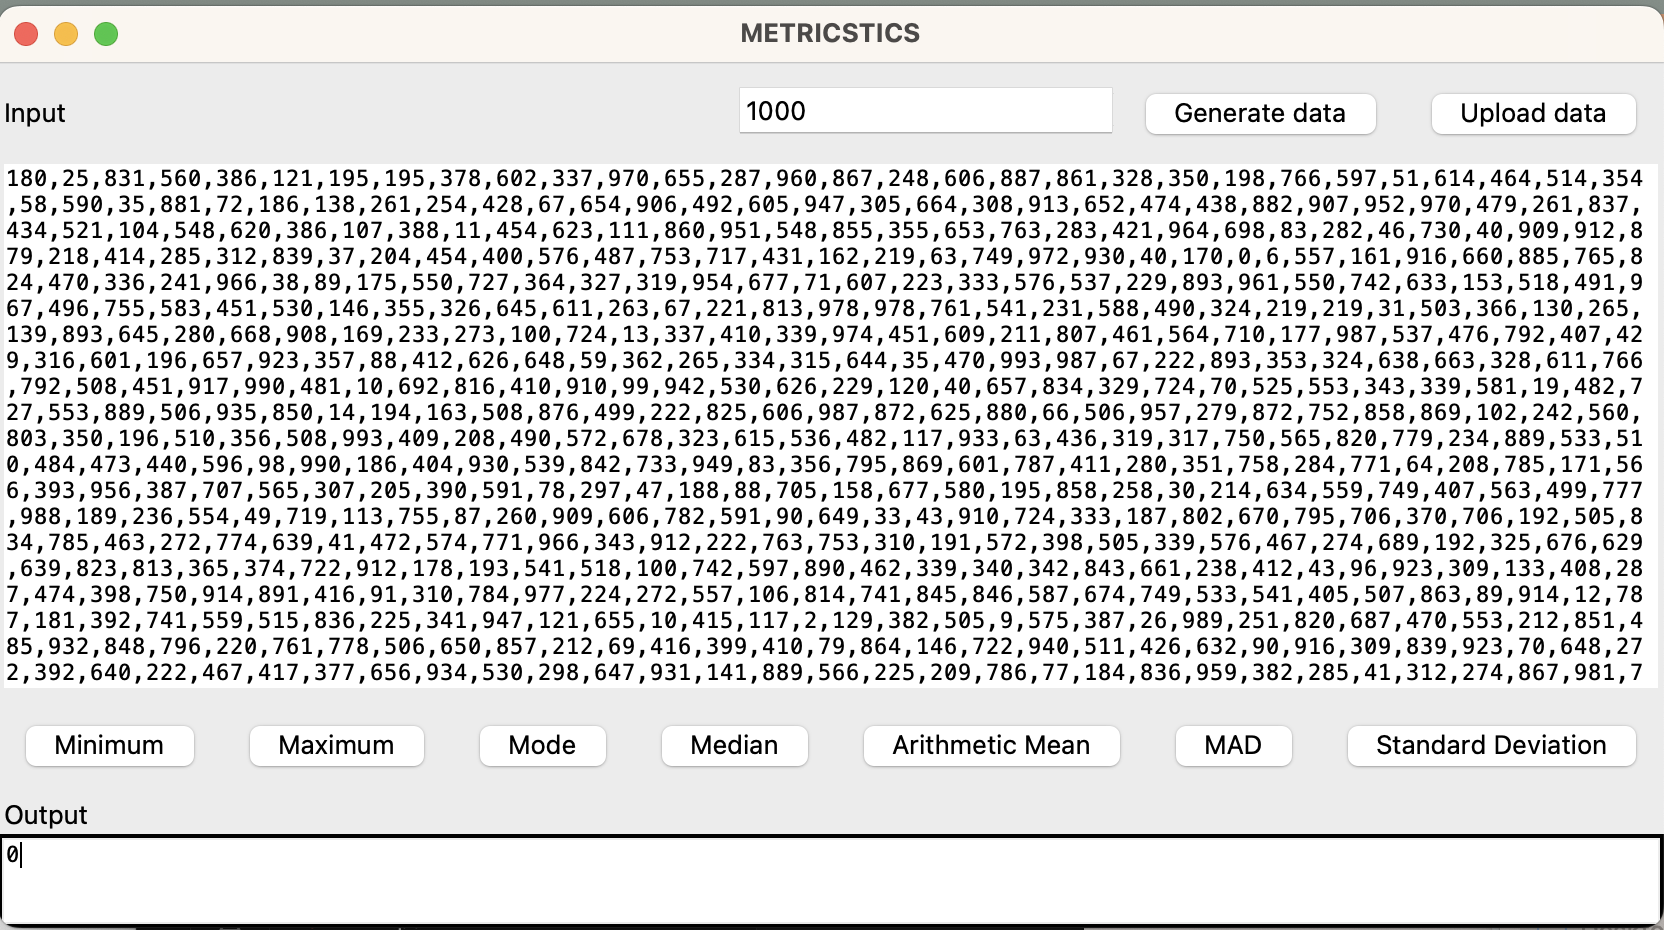
\includegraphics[width=11cm\textwidth]{images/random1_min.png}}\\
\hline
Max &   \raisebox{-\totalheight}{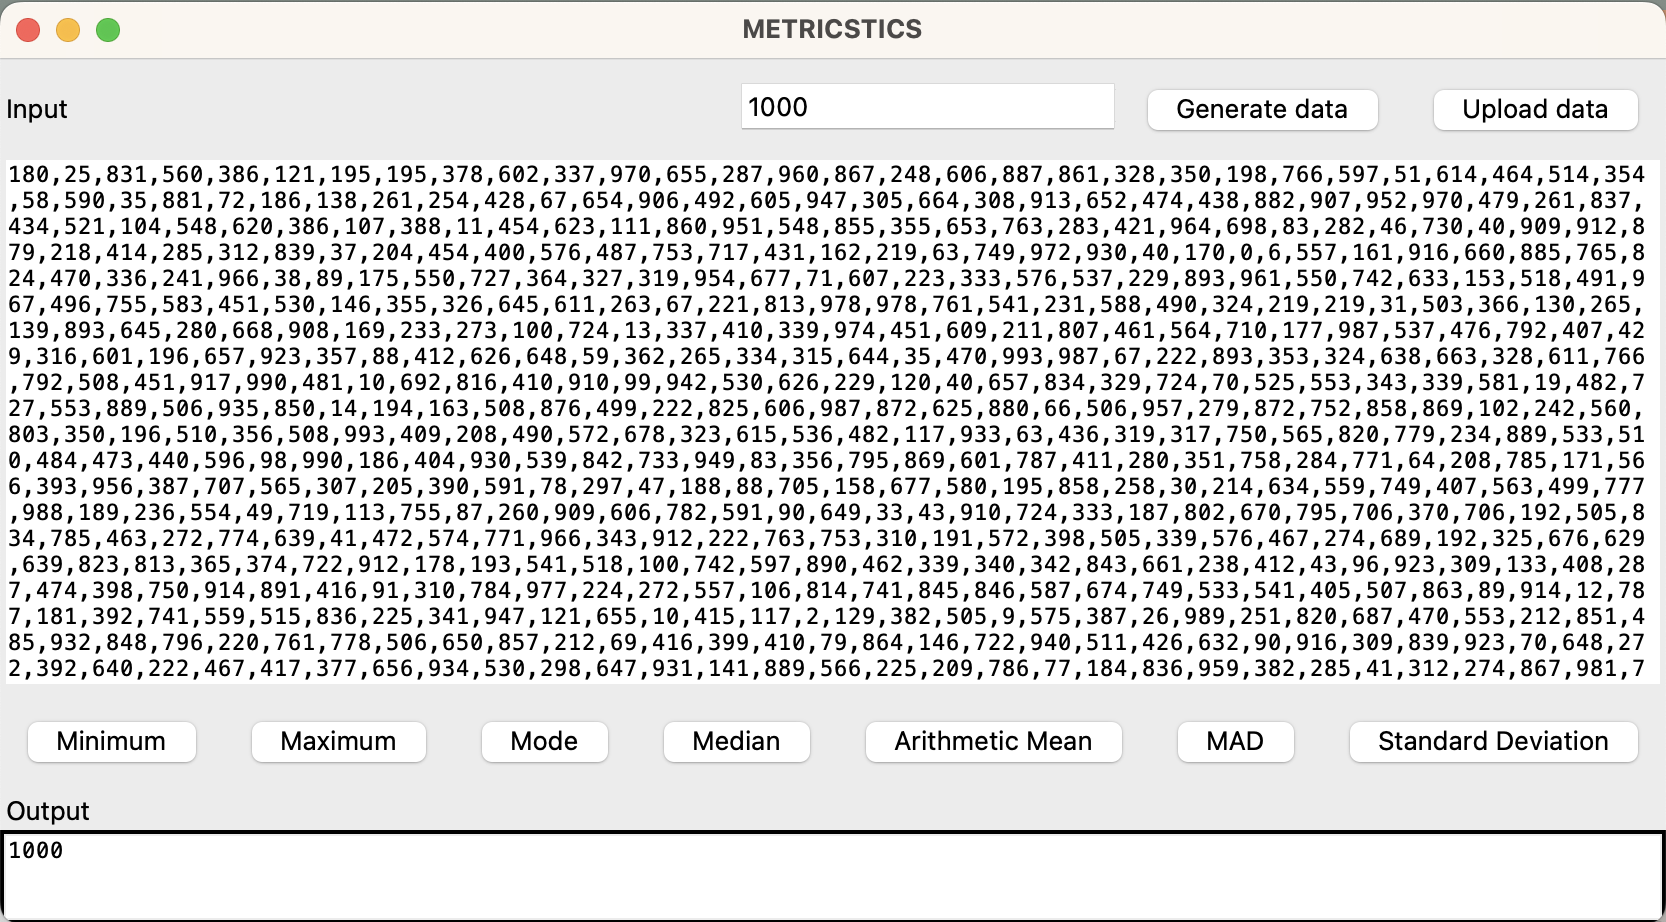
\includegraphics[width=11cm\textwidth]{images/random1_max.png}}\\
\hline
Mode &   \raisebox{-\totalheight}{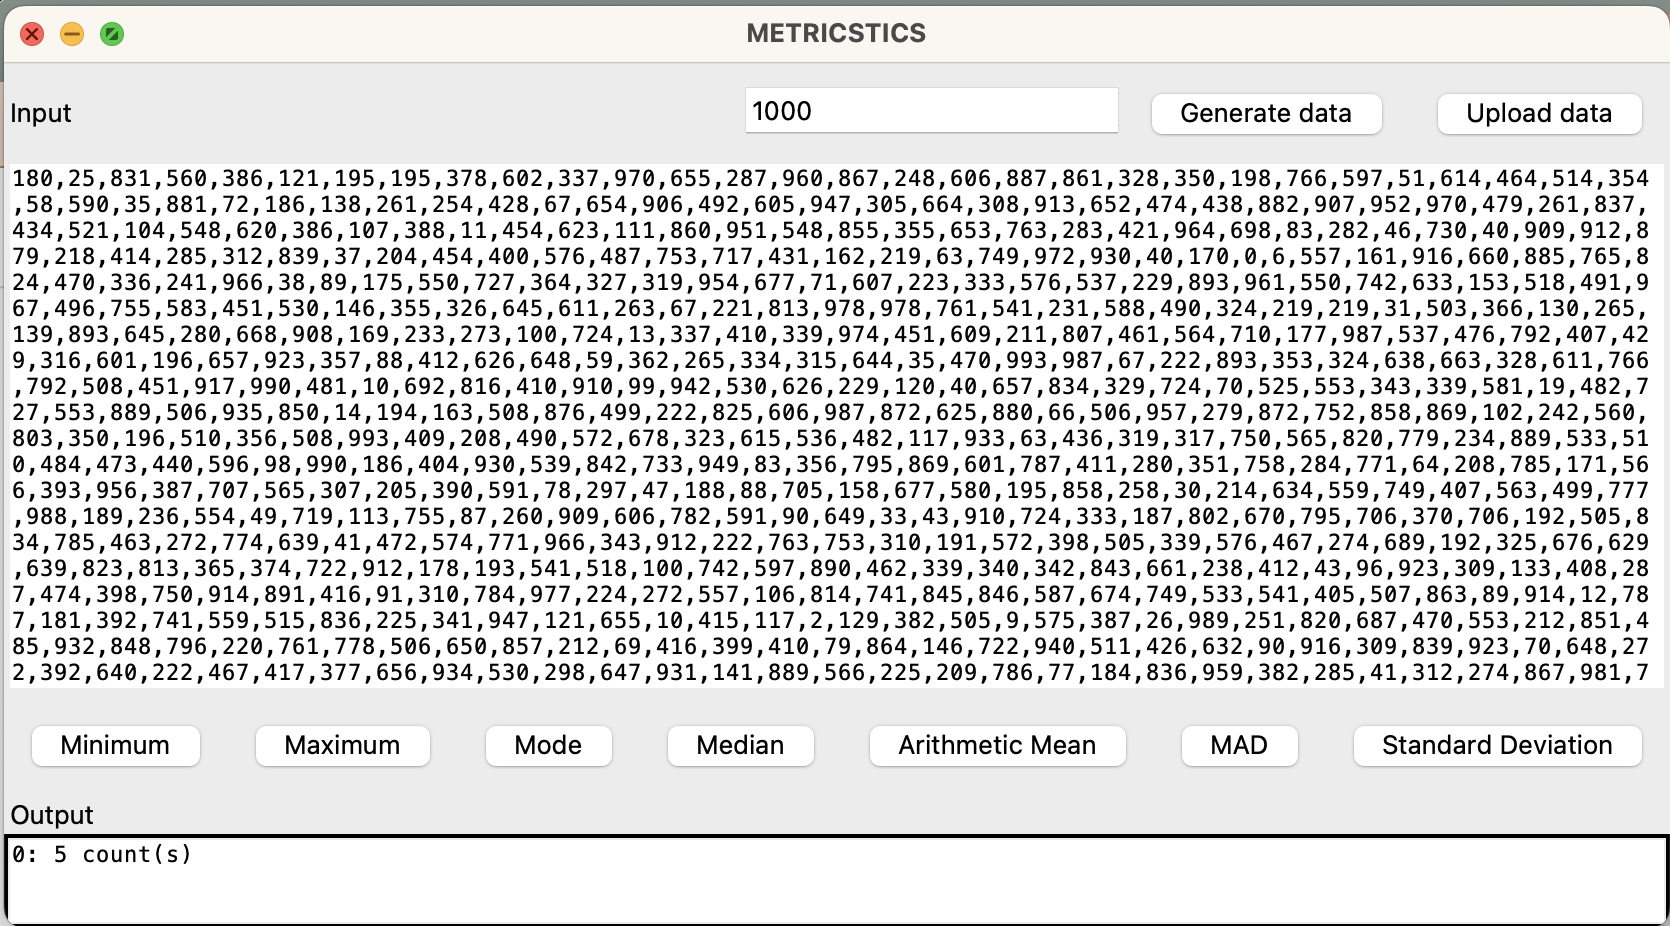
\includegraphics[width=11cm\textwidth]{images/random1_mode.png}}\\
\hline
Median &   \raisebox{-\totalheight}{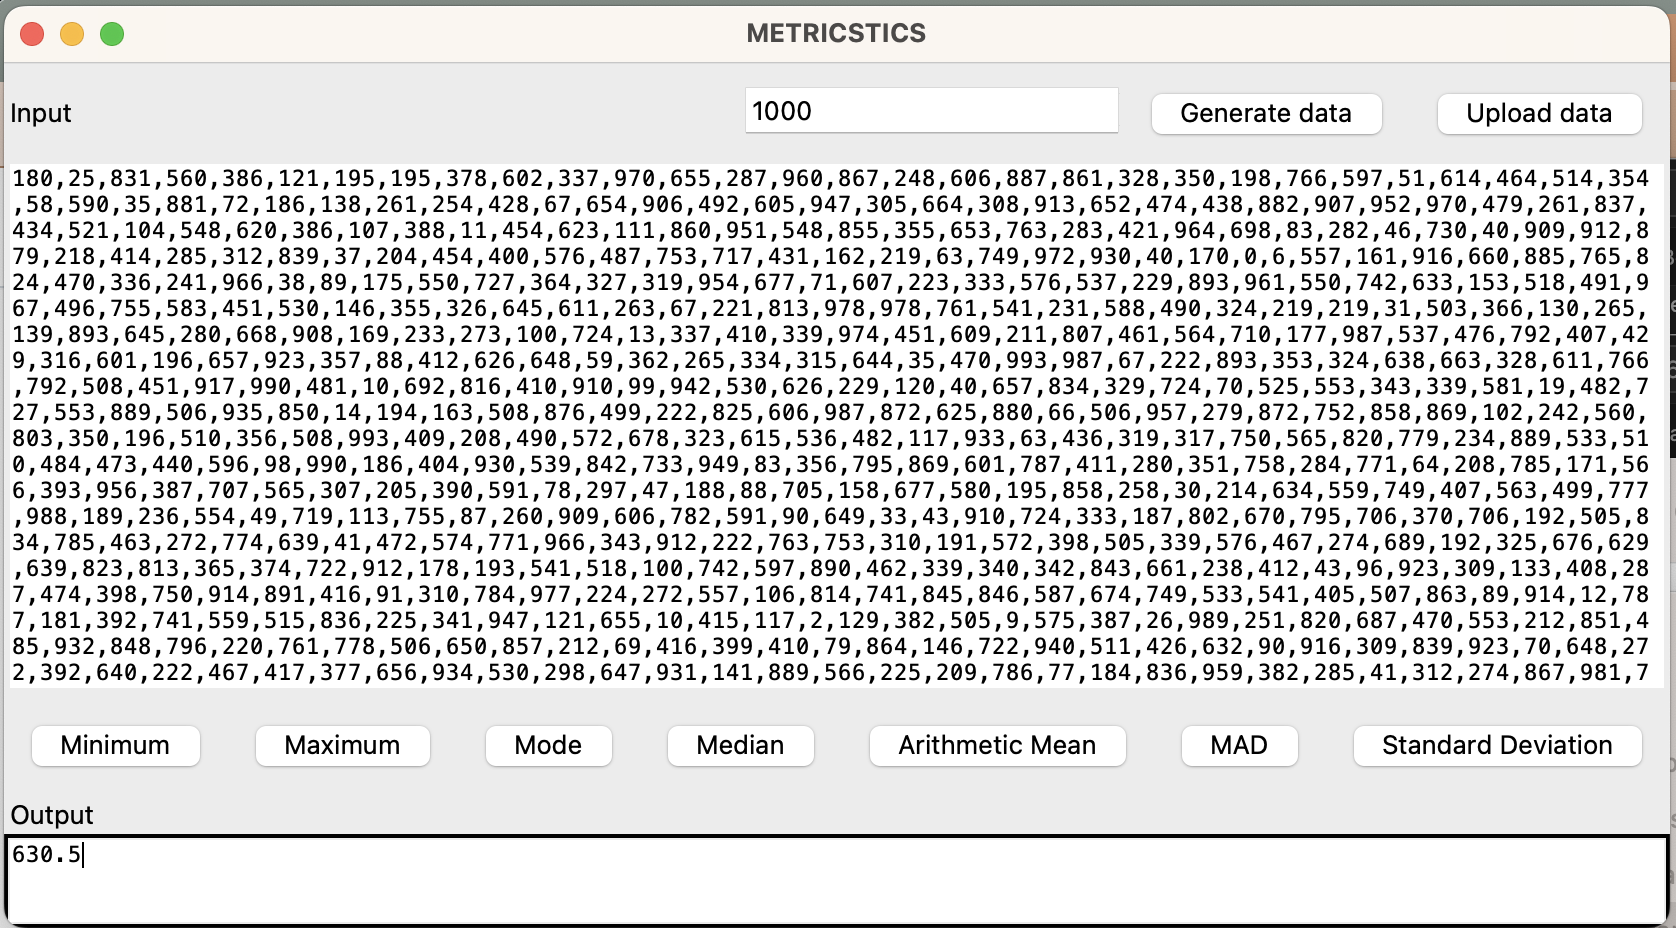
\includegraphics[width=11cm\textwidth]{images/random1_median.png}}\\
\hline
MAD &   \raisebox{-\totalheight}{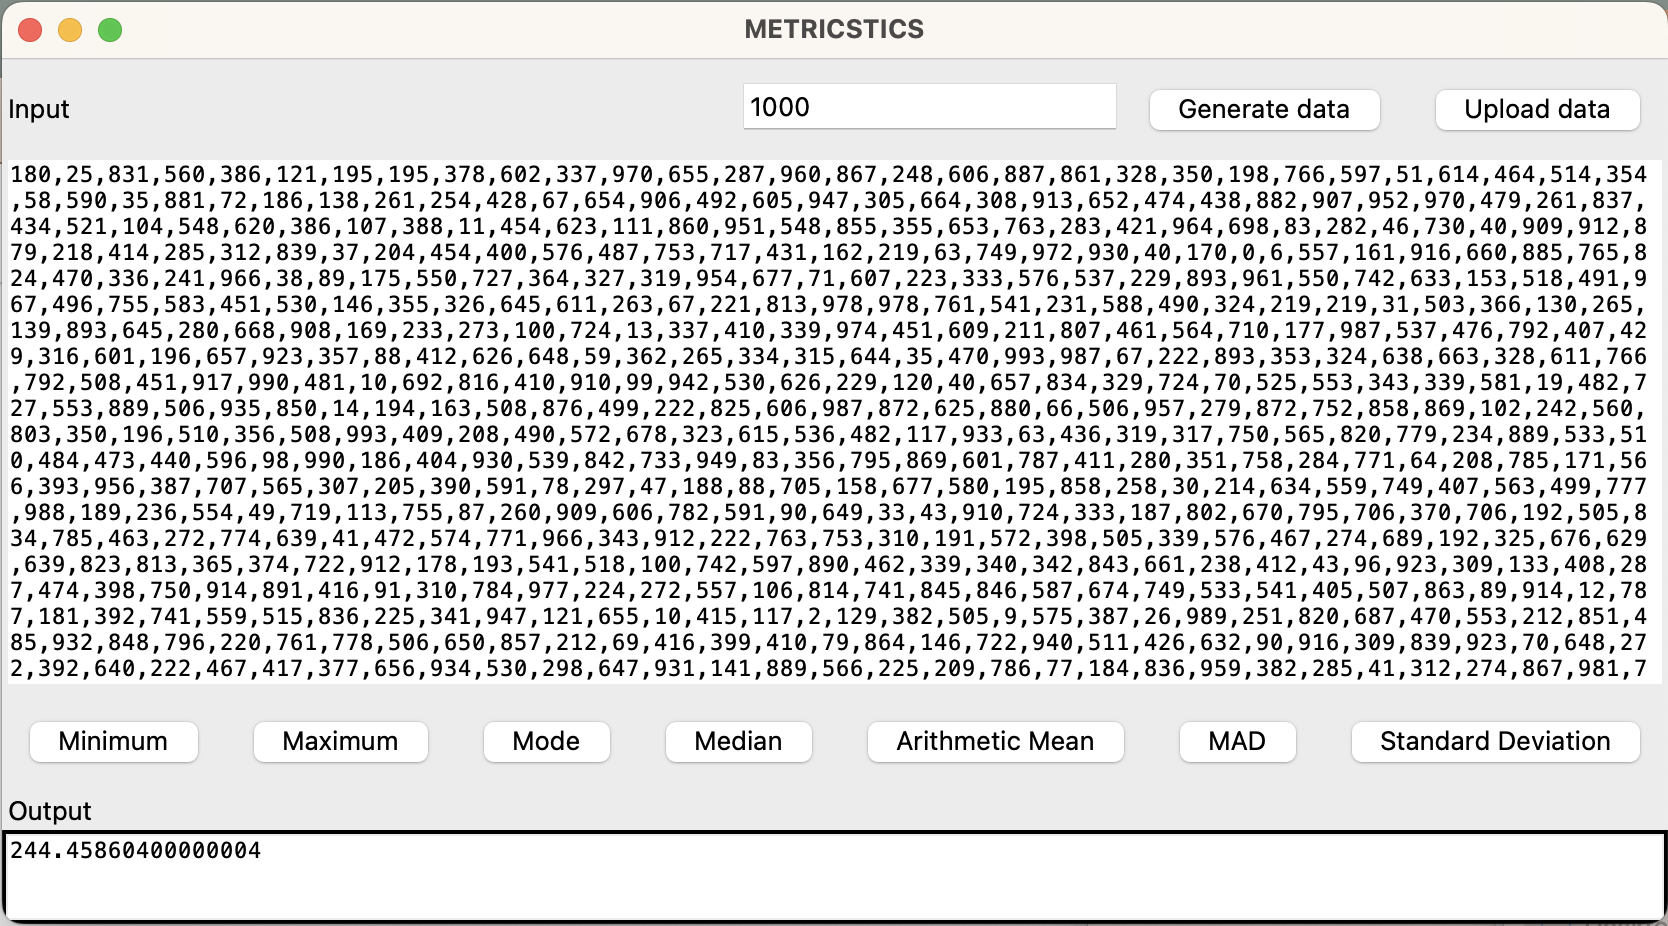
\includegraphics[width=11cm\textwidth]{images/random1_mad.png}}\\
\hline
Standard Deviation &   \raisebox{-\totalheight}{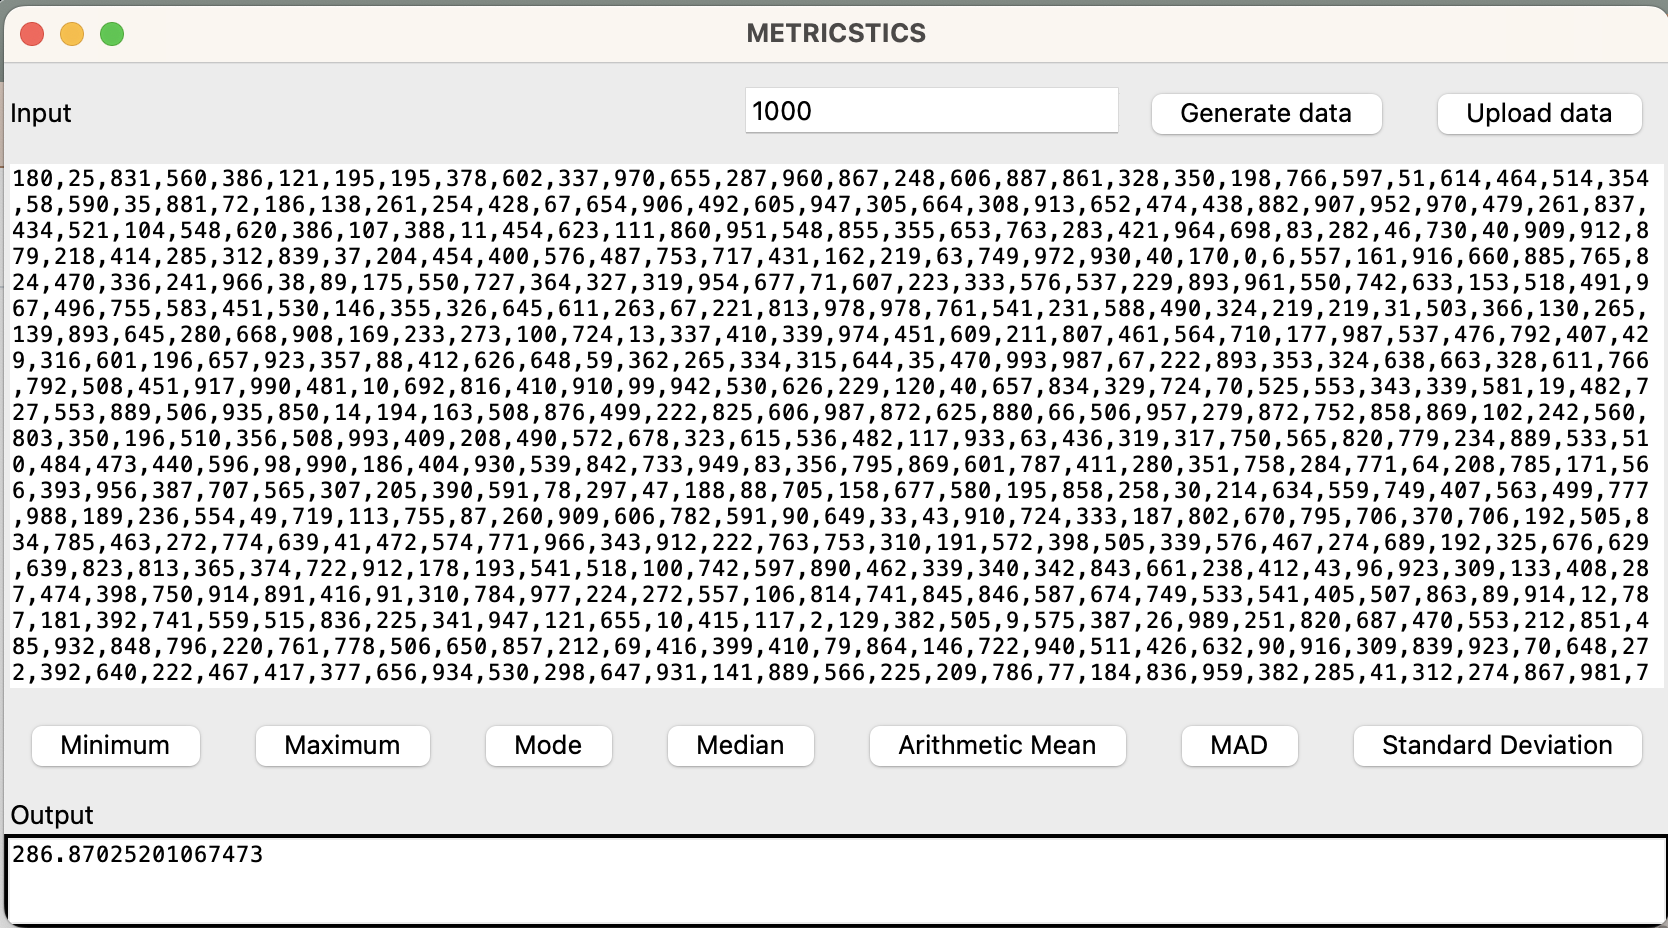
\includegraphics[width=11cm\textwidth]{images/random1_standarddeviation.png}}\\
\hline
\end{longtable}

\begin{longtable}{|l|l|}
\hline
\textbf{Test: Input 3} & Input from input3\_error.csv \\
\hline
Error input &   \raisebox{-\totalheight}{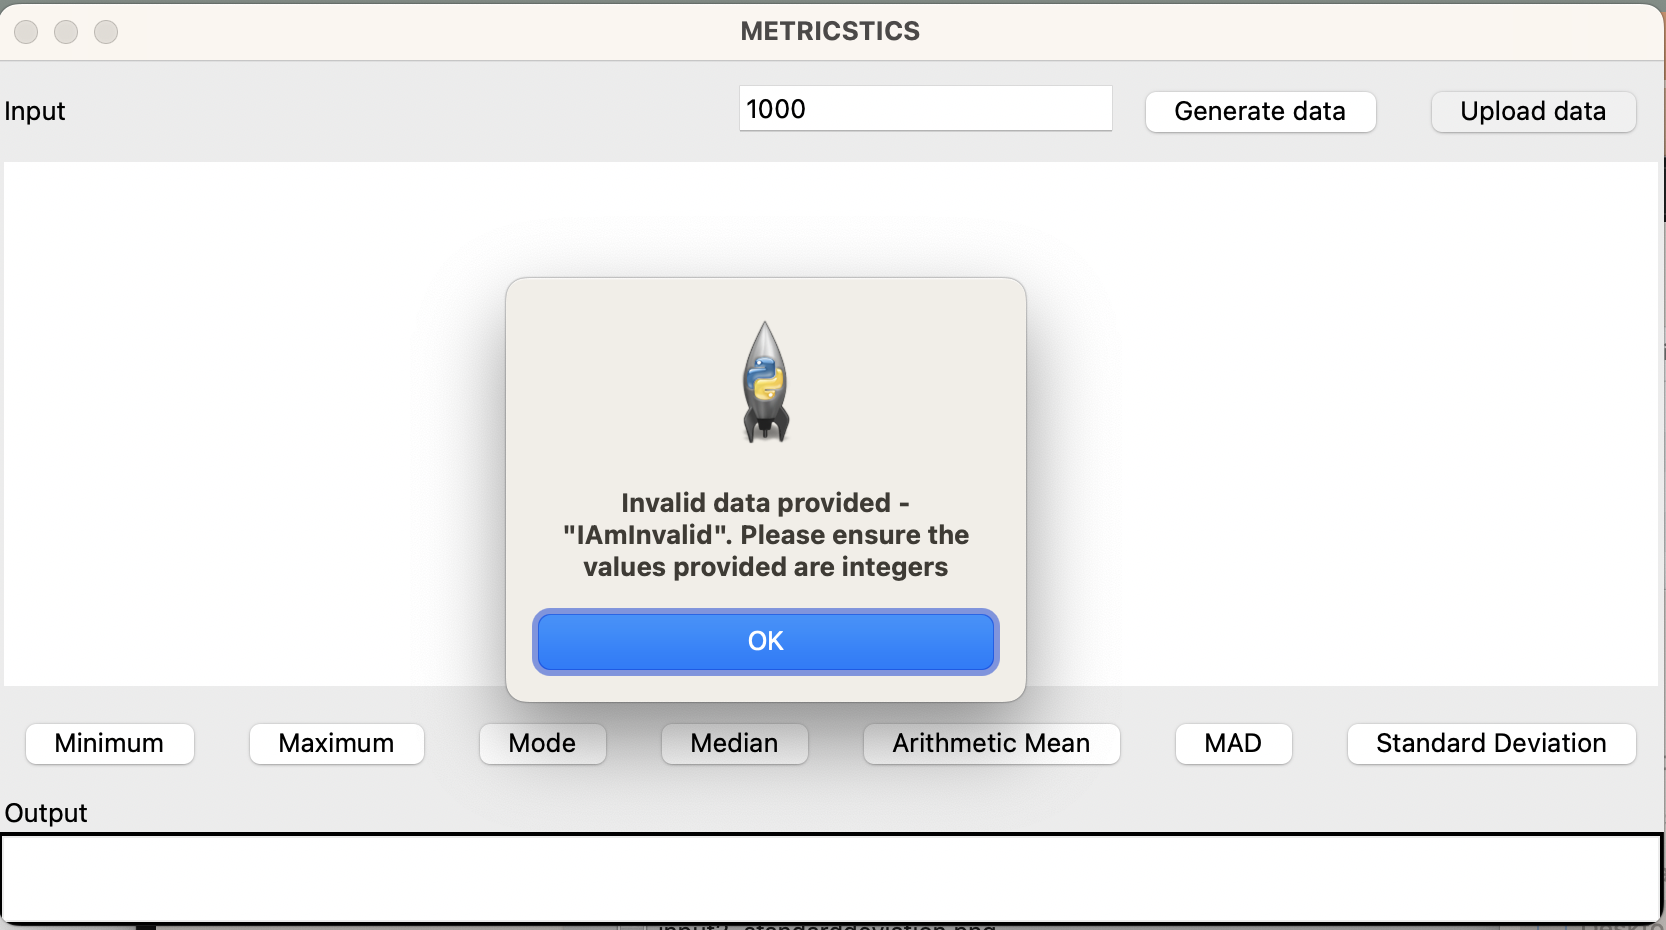
\includegraphics[width=11cm\textwidth]{images/input3_error.png}}\\
\hline
\end{longtable}

\pagebreak